% ECTA 2026 — Disentangling Density from Cycles
% Springer LNCS format. Double-blind submission.
\documentclass{llncs}

\usepackage{graphicx}
\usepackage{booktabs}
\usepackage{amsmath,amssymb}
\usepackage[T1]{fontenc}
\usepackage[hyphens]{url}
\usepackage{microtype}

% Figure path
\graphicspath{{figures/}}

\begin{document}

\title{Disentangling Density from Cycles\\in Multi-Agent Communication Topologies}
\author{[ANONYMOUS]}
\institute{[ANONYMOUS]}
\maketitle

\begin{abstract}
At least seven recent multi-agent systems enforce DAG communication topologies,
claiming that acyclic structure improves performance. We prove that these claims
rest on a methodological confound: for connected graphs with $n$ vertices and $m$
edges, the cycle rank $\beta_1 = m - n + 1$, so every comparison that varies
topology while varying edge count conflates cycle structure with density. To
escape this identity, we introduce directed simple cycle count $\kappa(D)$ as an
experimental variable that decorrelates from density---eight directed graph
families at constant $(n, m) = (8, 16)$ span $\kappa$ from 0 to 47. Across 240
controlled island model GA runs on OneMax, we find a significant main effect of
topology on diversity (ANOVA $p < 10^{-7}$, $\eta^2 = 0.17$) with Pearson
$r = -0.68$ between $\kappa$ and diversity at generation~30, with the effect
proving transient on OneMax. However, a supplementary NK
landscape pilot shows $14\times$ amplification at $K = 6$ ($\eta^2 = 0.69$
for diversity), confirming that topology effects scale with landscape
ruggedness. The existence of these effects at constant density demonstrates
that the DAG hegemony rests on confounded evidence, not controlled experiment.
\end{abstract}

%% ===================================================================
\section{Introduction}
\label{sec:intro}
%% ===================================================================

In island model genetic algorithms, the \emph{migration topology}---a graph
whose vertices are subpopulations and whose edges determine migration
routes---shapes diversity maintenance and convergence
speed~\cite{tomassini2005spatially,alba1999parallel}. Ring topologies maintain
diversity longer than complete graphs; sparse topologies slow premature
convergence~\cite{alba2002parallel,skolicki2005influence}. The open question is
not \emph{whether} topology matters but \emph{which topological property} is
operative. Yang et al.~\cite{yang2025topology} identify topology as the single
most underexplored dimension of MAS design, proposing nine research directions;
a recent survey formalises agent coordination as graph
computation~\cite{graphsaiagents2025}. Neither, however, identifies the
algebraic confound we expose below.

Recent LLM-based multi-agent systems (MAS) have intensified this question.
Seven major systems---GoAgent~\cite{goagent2026},
AgentConductor~\cite{agentconductor2026}, Graph-GRPO~\cite{graphgrpo2026},
OFA-MAS~\cite{ofamas2026}, G-Designer~\cite{gdesigner2025},
ARG-Designer~\cite{argdesigner2026}, and Dochkina et
al.~\cite{dochkina2026}---enforce or recommend DAG communication topologies.
Against this consensus, BIGMAS~\cite{bigmas2026} permits cycles,
Agent~Q-Mix~\cite{agentqmix2026} learns communication actions that create
2-cycles, and Puppeteer~\cite{puppeteer2025} discovers cyclic structures under
optimization pressure. The field is split, with no shared framework to
adjudicate.

The reason is algebraic. For any connected graph~$G$ with $n$ vertices and $m$
edges, the cycle rank $\beta_1(G) = m - n + 1$~\cite{hatcher2002algebraic}:
cycle count and edge count differ by a constant. Since Pearson correlation is
affine-invariant, $\rho(\beta_1, Y) = \rho(m, Y)$ for any outcome~$Y$. Every
comparison of ``cyclic'' versus ``acyclic'' topologies therefore simultaneously
varies density. The DAG hegemony and pro-cycle findings are both potentially
density effects in disguise.

We resolve this via directed graph theory. The simple directed cycle count
$\kappa(D)$ is not determined by $(n, m)$: two digraphs with $n = 8$, $m = 16$
can have 0 or 47 simple directed cycles. Across 240 runs (8~topology families,
30~seeds) at constant density, we find a significant main effect on diversity
($\eta^2 = 0.17$, $p < 10^{-7}$) with $r = -0.68$ between $\kappa$ and
diversity at generation~30.

The contributions are: \textbf{(1)}~a theorem proving the density--cycle
confound for connected undirected graphs; \textbf{(2)}~directed simple
cycle count $\kappa(D)$ as a density-independent experimental variable;
\textbf{(3)}~the first controlled experiment showing that directed cycle
structure ($\kappa$) has an independent effect on island model GA dynamics; and
\textbf{(4)}~NK landscape results showing $14\times$ amplification on
rugged landscapes.

%% ===================================================================
\section{Background}
\label{sec:background}
%% ===================================================================

\subsection{Island Model Evolutionary Algorithms}

In island model EAs, a population is partitioned into semi-isolated
subpopulations that evolve independently and exchange individuals via
migration~\cite{tomassini2005spatially}. The \emph{migration topology}
$G = (V, E)$ determines which islands may exchange migrants. The \emph{density}
of $G$ is $|E|/|V|$, the average number of connections per
island.\footnote{Some authors use $|E|/\binom{|V|}{2}$; the choice does not
affect the confound since both are affine in~$|E|$.} Sparse topologies
slow the spread of fit individuals, maintaining diversity; dense topologies
accelerate convergence but risk premature diversity
loss~\cite{alba2002parallel,skolicki2005influence}.

\subsection{Cycle Rank and the First Betti Number}

For a graph $G$ with $n$ vertices, $m$ edges, and $c$ connected components, the
first Betti number is $\beta_1(G) = m - n + c$.
For connected graphs ($c = 1$), $\beta_1 = m - n + 1$. Geometrically, $\beta_1$
counts independent cycles: a spanning tree uses $n-1$ edges, and each additional
edge closes exactly one independent
cycle~\cite{hatcher2002algebraic}. Prior work reports correlations
between $\beta_1$ and fitness convergence, but as Section~\ref{sec:confound}
shows, these are algebraically indistinguishable from density effects.

\subsection{Directed Graphs and Simple Cycle Count}

A digraph $D = (V, A)$ has arcs (ordered pairs) rather than edges. The
\emph{simple directed cycle count} $\kappa(D)$ is the number of elementary
directed cycles in $D$. Unlike $\beta_1$, which for connected graphs is
determined by $n$ and $m$, $\kappa(D)$ depends on the specific arc arrangement.
Enumeration uses Johnson's algorithm~\cite{johnson1975finding}.

%% ===================================================================
\section{The Density--Cycle Confound}
\label{sec:confound}
%% ===================================================================

\begin{theorem}[Cycle rank--density identity]
\label{thm:confound}
Let $G = (V, E)$ be a connected graph with $|V| = n$ and $|E| = m$. Then
$\beta_1(G) = m - n + 1$.
\end{theorem}

\begin{proof}
Any spanning tree of $G$ uses $n - 1$ edges; each remaining edge closes exactly
one independent cycle. The result follows from the Euler characteristic
$\chi = n - m = 1 - \beta_1$ for connected 1-dimensional simplicial complexes.
\end{proof}

\begin{corollary}
\label{cor:pearson}
For connected graphs with fixed $n$, $\beta_1$ and $m$ differ by the constant
$n - 1$. Pearson correlation is invariant under affine transformation, so
$\rho(\beta_1, Y) = \rho(m, Y)$ for any outcome variable~$Y$.
\end{corollary}

The methodological consequence: \emph{any experiment comparing connected
topologies on a fixed node count cannot distinguish ``cycles affect
performance'' from ``edge count affects performance.''}
Table~\ref{tab:confound} surveys seven systems exhibiting this confound.

\begin{table}[t]
\centering
\caption{Systems enforcing the DAG constraint. All vary $\beta_1$ and density simultaneously.}
\label{tab:confound}
\small
\resizebox{\columnwidth}{!}{%
\begin{tabular}{lll}
\toprule
\textbf{System} & \textbf{Claim} & \textbf{Confound} \\
\midrule
GoAgent~\cite{goagent2026}
  & DAG enables tractable CIB
  & DAG vs.\ dense baseline varies $\beta_1$ and $m$ \\
Graph-GRPO~\cite{graphgrpo2026}
  & Learned DAGs beat complete graphs
  & Complete = max density and max $\beta_1$ \\
OFA-MAS~\cite{ofamas2026}
  & Sparse communication improves efficiency
  & Pruning reduces $m$ and $\beta_1$ in lockstep \\
G-Designer~\cite{gdesigner2025}
  & Moderate connectivity best
  & No density-controlled baseline \\
AgentConductor~\cite{agentconductor2026}
  & DAG topology evolution for code generation
  & Evolves DAGs only; cyclic alternatives never tested \\
ARG-Designer~\cite{argdesigner2026}
  & Autoregressive DAG generation
  & DAG constraint baked into generative model \\
Dochkina et al.~\cite{dochkina2026}
  & Sparse beats dense; capability moderates
  & Sparsity and acyclicity confounded in all 25K runs \\
\bottomrule
\end{tabular}}
\end{table}

\subsection{The Directed Escape}

Theorem~\ref{thm:confound} applies to homological cycle rank. For directed
graphs, the simple cycle \emph{count} $\kappa(D)$ is combinatorial, not
homological: it depends on arc arrangement, not cycle space dimension.
We constructed eight families at constant $(n, m) = (8, 16)$ with $\kappa$
ranging from 0 to 47. Among strongly connected members alone, $\kappa$ spans
10 to 47---a $4.7\times$ variation at strictly constant density and identical
directed rank~9.

%% ===================================================================
\section{Experimental Design}
\label{sec:design}
%% ===================================================================

All experiments below use the directed simple cycle count $\kappa(D)$, not the
homological $\beta_1$, as the independent variable.

\subsection{Graph Families}

Table~\ref{tab:families} describes the eight directed graph families, all with
$n = 8$ vertices and $m = 16$ arcs (density $m/n = 2.0$ held constant). Cycle
counts were verified by exhaustive enumeration via Johnson's
algorithm~\cite{johnson1975finding}.

\begin{table}[t]
\centering
\caption{Eight directed graph families at constant density ($n=8$, $m=16$).
$\kappa$ = directed simple cycle count. SC = strongly connected.}
\label{tab:families}
\begin{tabular}{llcc}
\toprule
Family & Description & $\kappa$ & SC \\
\midrule
\texttt{dag-layer}      & 3-layer forward hierarchy                  &  0 & No  \\
\texttt{dag-wide}       & Fan-out; single coordinator broadcasts     &  0 & No  \\
\texttt{lowcyc-1}       & \texttt{dag-layer} + one feedback arc      &  3 & No  \\
\texttt{bidir-ring}     & Forward and backward directed 8-ring       & 10 & Yes \\
\texttt{two-cliques}    & Two directed 4-cycles with cross-chords    & 14 & No  \\
\texttt{mesh-cyclic}    & $2\times4$ grid with bidirectional verticals & 20 & Yes \\
\texttt{dense-triangles}& Overlapping directed triangles + skip-2    & 29 & Yes \\
\texttt{ring-skip2}     & Ring $i{\to}i{+}1$ plus $i{\to}i{+}2$ (mod 8) & 47 & Yes \\
\bottomrule
\end{tabular}
\end{table}

\subsection{Island Model GA}

Each vertex hosts one subpopulation of 50 individuals (400 total). The fitness
function is OneMax on $L = 100$-bit strings:
$f(\mathbf{x}) = L^{-1}\sum_{k=1}^{L} x_k \in [0, 1]$. OneMax is unimodal,
chosen so that any topology effect is structural, not landscape-specific.

Selection is tournament ($k = 3$); crossover is uniform ($p = 0.5$/locus);
mutation is bit-flip at rate $p_m = 1/L = 0.01$ per bit. Every 10 generations,
the 5 fittest individuals on each island migrate along outgoing arcs, replacing
the 5 weakest (synchronous migration). All families share density
$16/8 = 2.0$. Runs last 500 generations.

\subsection{Metrics and Statistical Analysis}

\paragraph{Diversity.} Mean pairwise normalised Hamming distance across all 400
individuals:
\[
  D(t) = \frac{1}{\binom{N}{2}} \sum_{i < j}
    \frac{d_H(\mathbf{x}_i, \mathbf{x}_j)}{L},
\]
estimated from 20 randomly sampled pairs when $N > 20$.

\paragraph{Analysis.} Pearson $r$ between $\kappa$ and each metric at
generations 30, 60, and 100. One-way ANOVA ($\alpha = 0.05$) with topology as
factor; effect size $\eta^2$; post-hoc Mann--Whitney~$U$ with Bonferroni
correction. Because all families share $m = 16$, $r(\text{density}, Y) = 0$
identically. Each topology runs with 30 seeds ($240$ total). Implementation:
Haskell; cycle counts pre-computed via Johnson's algorithm in Python.

\subsection{NK Landscape Pilot}

To test scaling with landscape difficulty, we ran a pilot on NK
landscapes~\cite{kauffman1993origins} ($N = 100$, adjacent neighbours,
$K \in \{0, 4, 6\}$, fixed seed). Three topologies spanning $\kappa$:
dag-layer (0), bidir-ring (10), ring-skip2 (47); 10 seeds per condition
($90$ runs).

%% ===================================================================
\section{Results}
\label{sec:results}
%% ===================================================================

\subsection{Topology Significantly Affects Diversity and Fitness}

One-way ANOVA yields $F(7, 232) = 6.90$, $p = 1.85 \times 10^{-7}$ at
generation~30; Kruskal--Wallis corroborates ($H = 38.53$,
$p = 2.40 \times 10^{-6}$). Effect sizes: $\eta^2 = 0.17$ (diversity),
$\eta^2 = 0.24$ (fitness)---medium-to-large. Density is constant by
construction, so $r(\text{density}, Y) = 0$ identically.

\subsection{Cycle Count Negatively Predicts Diversity}

Figure~\ref{fig:scatter} shows $\kappa(D)$ against mean diversity at
generation~30. Pearson $r = -0.681$ ($r^2 = 0.46$, $p = 0.063$ on 6~df);
the marginal $p$ reflects only 8 topology-level points, while the 240-run
ANOVA confirms the effect. Post-hoc Bonferroni contrasts: dag-wide
($\kappa = 0$) differs from all $\kappa \geq 10$ topologies ($p < 0.001$).

\subsection{The Effect Is Transient}

The temporal profile (Figures~\ref{fig:trajectories}--\ref{fig:effectsize}):
at generation~30, $r = -0.681$, $\eta^2 = 0.17$; at generation~50,
$r = 0.838$ for fitness ($p = 0.009$; higher $\kappa$ slows convergence,
yielding lower fitness at generation~50); by generation~100, $|r| < 0.10$,
$\eta^2 = 0.002$. OneMax is unimodal, so all topologies eventually converge;
$\kappa$ affects the \emph{rate} of diversity loss, not the outcome.
DAG families converge fastest; ring-skip2 ($\kappa = 47$) sustains diversity
longest. The bidirectional ring does not fall monotonically, suggesting cycle
\emph{length distribution} may contribute independently~\cite{cycrak2024}.

\begin{figure}[t]
  \centering
  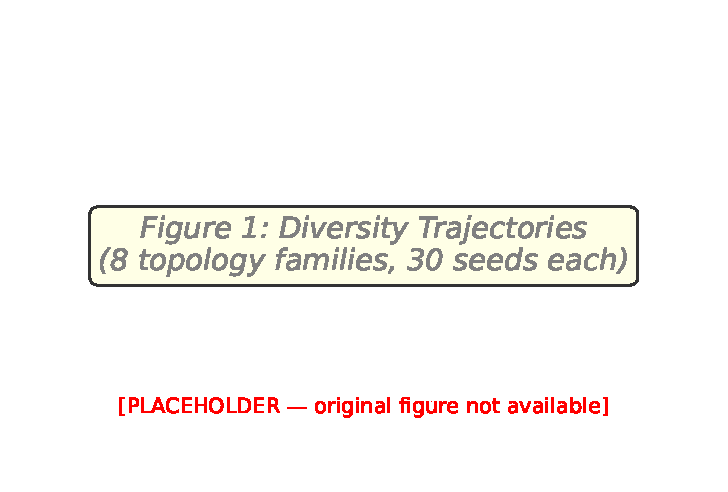
\includegraphics[width=0.82\textwidth]{fig1_diversity_trajectories.pdf}
  \caption{Mean diversity trajectories ($\pm$ 1 SE) for 8 topology families
  (30 seeds each). DAG families converge fastest; ring-skip2 ($\kappa = 47$)
  sustains diversity longest.}
  \label{fig:trajectories}
\end{figure}

\begin{figure}[t]
  \centering
  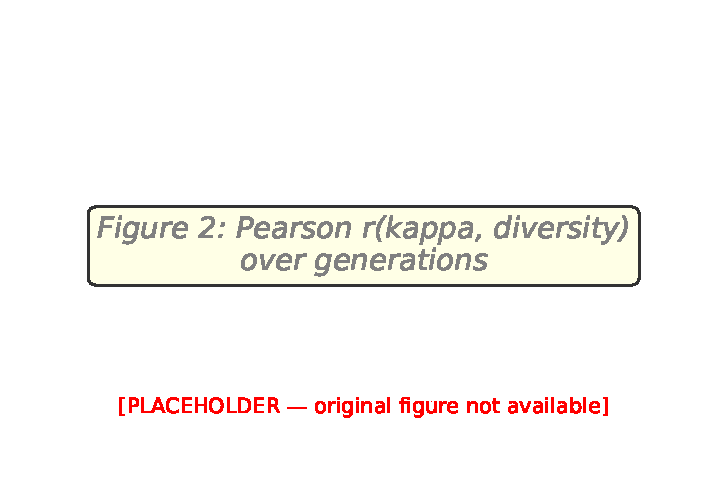
\includegraphics[width=0.7\textwidth]{fig2_correlation_over_time.pdf}
  \caption{Pearson $r(\kappa, \text{diversity})$ over generations. Peak at
  gen.\ 20--50; decay by gen.\ 100.}
  \label{fig:correlation}
\end{figure}

\begin{figure}[t]
  \centering
  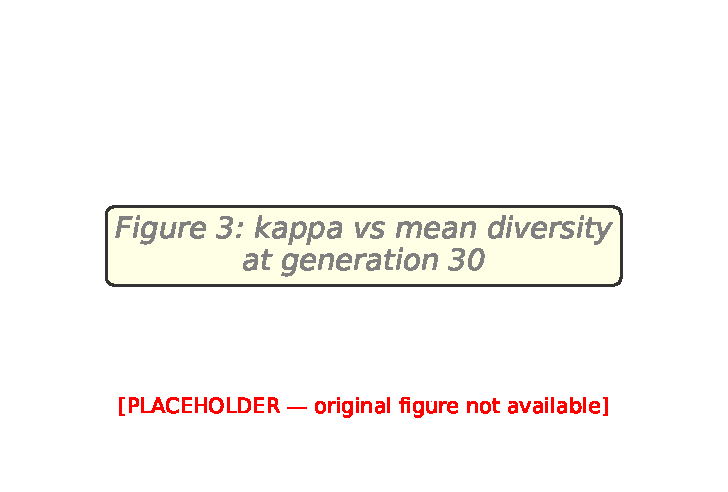
\includegraphics[width=0.7\textwidth]{fig3_scatter_gen30.pdf}
  \caption{$\kappa$ vs.\ mean diversity at gen.\ 30. $r = -0.681$ ($p = 0.063$, 6 df).}
  \label{fig:scatter}
\end{figure}

\begin{figure}[t]
  \centering
  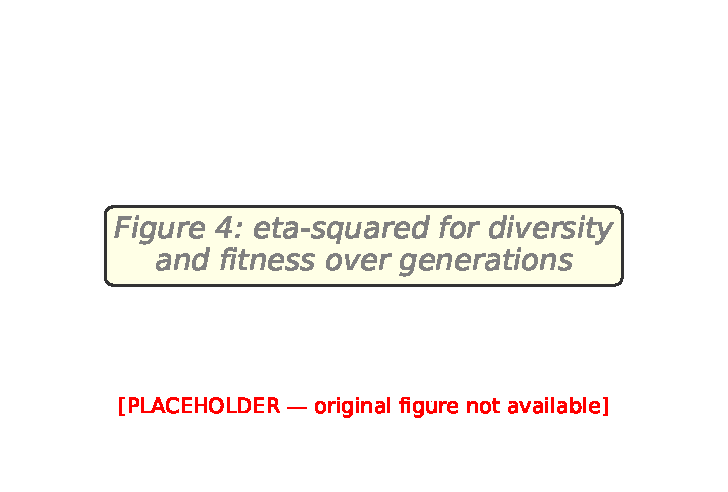
\includegraphics[width=0.7\textwidth]{fig4_effect_size.pdf}
  \caption{$\eta^2$ for diversity and fitness over generations. Peak near gen.\ 30; decay by gen.\ 100.}
  \label{fig:effectsize}
\end{figure}

\subsection{Topology Effect Scales with Landscape Ruggedness}

Figure~\ref{fig:nk} shows $\eta^2$ for diversity increasing monotonically
with $K$: from $0.049$ ($K = 0$) to $0.445$ ($K = 4$) and $0.686$
($K = 6$, both $p < 10^{-3}$) at generation~200. Fitness follows:
$\eta^2 = 0.001, 0.337, 0.349$. On the rugged $K = 6$ landscape, nearly
70\% of diversity variance is explained by topology---a $14\times$
amplification over $K = 0$. The $K = 0$ control confirms these are genuine
topology--landscape interactions.

High-$\kappa$ topologies slow allele propagation, extending exploration.
On OneMax this merely delays convergence; on rugged landscapes, sustained
diversity prevents premature trapping. Ring-skip2 ($\kappa = 47$) maintains
highest diversity but not highest fitness at $K = 6$---bidir-ring
($\kappa = 10$) achieves marginally better fitness, suggesting a Goldilocks
effect. HERA~\cite{hera2026} independently converges to ``compact chains
with strategically preserved cycles''---intermediate $\kappa$ under
optimization pressure.

\begin{figure}[t]
  \centering
  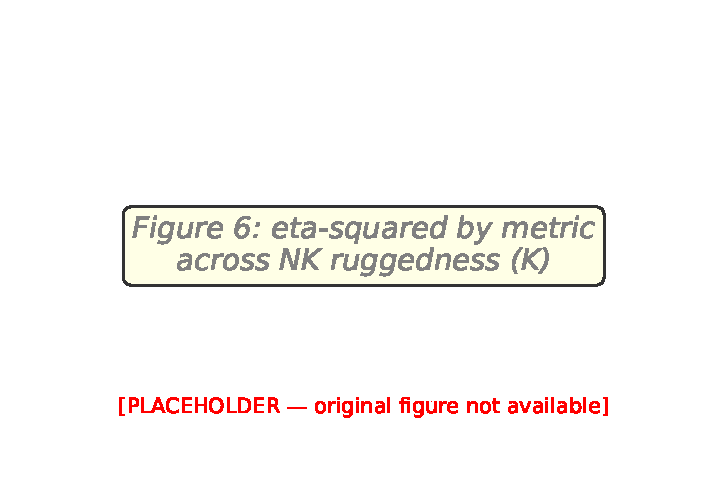
\includegraphics[width=0.7\textwidth]{fig6_nk_effect_size.pdf}
  \caption{$\eta^2$ by metric across NK ruggedness ($K$) at gen.\ 200.
  Topology explains $<5\%$ at $K = 0$ but $\sim$70\% of diversity at $K = 6$.
  Dashed: Cohen's thresholds. $^{**}p < 0.01$; $^{***}p < 0.001$.}
  \label{fig:nk}
\end{figure}

%% ===================================================================
\section{Discussion}
\label{sec:discussion}
%% ===================================================================

At constant density, $\kappa(D)$ explains 17\% of diversity variance and 24\%
of fitness variance at generation~30---medium-to-large effects on a landscape
deliberately chosen to be easy. We interpret the temporal profile as
\emph{cycle-mediated exploration}: feedback loops slow the propagation of
dominant alleles, extending the period during which subpopulations maintain
independent search. On OneMax, selection pressure eventually overwhelms this
phase. The NK pilot confirms: $\eta^2$ rises from 0.049 ($K = 0$) to 0.686
($K = 6$), sustained above 0.50 at generation~500 while collapsing to near
zero for $K = 0$.

\paragraph{Diversity as the primary channel.}
Across both experiments, diversity is most sensitive to topology. On NK
landscapes, diversity $\eta^2 = 0.686$ while best-fitness $\eta^2 < 0.10$.
Cycles operate through population-level diversity maintenance rather than direct
fitness improvement. Practitioners should monitor diversity, not just fitness,
when evaluating communication topologies.

The implications for MAS design are immediate. The systems in
Table~\ref{tab:confound} concluded DAGs outperform, but by
Theorem~\ref{thm:confound} their experiments compared sparse to dense. The
correct conclusion is that \emph{sparser communication is cheaper}, not that
cycles are harmful. Abbott et al.~\cite{abbott2025streamability} formalise the
cost side: DAGs are streamable (linear execution), while cycles require fixpoint
iteration. Our experiments quantify the \emph{benefit} side---sustained
diversity on rugged landscapes---completing a cost-benefit framework for
topology choice.

Figure~\ref{fig:foster} illustrates the confound concretely. We ran the
same island model GA on 13 cubic symmetric graphs from the Foster
census~\cite{foster1988census} ($n = 4$ to $30$, 30 seeds each). Because
every 3-regular graph on $n$ vertices has $m = 3n/2$ edges, the cycle
rank $\beta_1 = n/2 + 1$, and the density $m/n = 3/2$---all three
quantities are affine in~$n$, hence perfectly collinear. The left panel
plots diversity against~$n$ (increasing trend); the right plots the
\emph{same data} against density $m/\binom{n}{2}$ (decreasing trend).
Both narratives are the same regression---the trap
Theorem~\ref{thm:confound} predicts. Only constant-density experiments
break the degeneracy. As a positive control, the Dodecahedron and Desargues
graphs share $n = 20$, $\beta_1 = 11$, density $3/19$; Mann--Whitney finds no
significant difference ($p = 0.615$), confirming that graphs matched on all
confounded variables produce indistinguishable dynamics.

\begin{figure}[t]
  \centering
  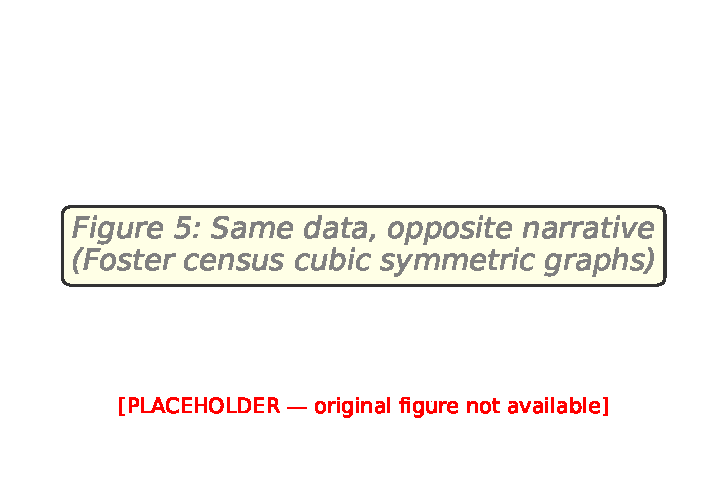
\includegraphics[width=0.82\textwidth]{fig5_foster_same_data.pdf}
  \caption{Same data, opposite narrative. Left: diversity vs.\ $n$. Right:
  diversity vs.\ density $m/\binom{n}{2}$. 13 Foster census cubic symmetric
  graphs ($n = 4$--$30$, 30 seeds). For 3-regular graphs, $\beta_1$, $m$,
  $n$ are collinear---causal attribution is underdetermined.}
  \label{fig:foster}
\end{figure}

\paragraph{Limitations.}
First, $n = 8$ islands is small; scaling experiments on larger graph families
are needed (the Foster sweep uses up to $n = 30$ but cannot escape the
density confound within the 3-regular family). Second, the Pearson correlation
is marginal ($p = 0.063$) on 8 topology-level points, though significant at
generation~50 ($r = 0.838$, $p = 0.009$) and corroborated by the 240-run
ANOVA ($p < 10^{-7}$). Third, the NK pilot uses only 3 of 8 topologies and
10 seeds; a full-factorial experiment is needed for generality.

%% ===================================================================
\section{Related Work}
\label{sec:related}
%% ===================================================================

\paragraph{Learned and adaptive topologies.}
Puppeteer~\cite{puppeteer2025} trains an RL orchestrator that discovers
``compact, cyclic reasoning structures'' on hard tasks, outperforming
DAG-constrained MacNet~\cite{macnet2025}. Cycles \emph{emerge} under
optimization pressure, but no topological metric ($\beta_1$, $\kappa$) is
computed and no ablation separates cycles from density. By
Theorem~\ref{thm:confound}, their evidence is exactly the confound our
experiment resolves. HERA~\cite{hera2026} is the first system to explicitly
track cycle count during topology evolution, converging to ``compact chains
with strategically preserved cycles''---intermediate $\kappa$ under optimization
pressure. Agent~Q-Mix~\cite{agentqmix2026} learns six communication actions
via QMIX, including a \texttt{debate\_check} action that creates directed
2-cycles; it is the most topology-aware RL-based system to date.
Our theorem explains why intermediate cycle counts work.

\paragraph{Large-scale studies.}
Lynch et al.~\cite{clocksystems2026} show that graph-parameterised
clock systems constrain representable behaviours to paths in~$G$: DAGs
permit only acyclic execution. Dochkina et al.~\cite{dochkina2026}
(25K+ runs) find sparse/acyclic outperforms dense/cyclic with
capability-moderated crossover. By Theorem~\ref{thm:confound}, this is
a density comparison; our experiment provides the controlled condition.

\paragraph{Cycle structure.}
CycRak~\cite{cycrak2024} shows short-cycle centrality outperforms eigenvector
centrality for diffusion, suggesting cycle \emph{length distribution} governs
propagation---consistent with our non-monotonic bidir-ring result.

%% ===================================================================
\section{Conclusion}
\label{sec:conclusion}
%% ===================================================================

For connected graphs with fixed vertex count, cycle rank $\beta_1$ and edge
count $m$ differ by a constant (Theorem~\ref{thm:confound}). Every prior
comparison of cyclic versus acyclic topologies is therefore confounded. We
escape this by moving to directed graphs, where $\kappa(D)$ is not determined
by $(n, m)$. Across 240 runs at constant density, $\kappa$ predicts diversity
($\eta^2 = 0.17$, $p < 10^{-7}$) and fitness ($\eta^2 = 0.24$). The effect is
transient on OneMax but a $14\times$ amplification at NK $K = 6$ confirms
scaling with landscape difficulty. Future work should pursue full-factorial NK
experiments, $\kappa$--capability interaction, and $\kappa$ as a practical
topology design heuristic---precisely the directions called for by recent
position papers~\cite{yang2025topology}.

%% ===================================================================
\bibliographystyle{splncs04}
\bibliography{references}

\end{document}
